\section{Largest and smallest of an array}
\subsection{Aim}
To find the largest and smallest of 8-bit numbers

\subsection{Code}
\begin{lstlisting}
ORG 0000H

MOV DPTR, #100H
MOV R0, #08H
MOV R1, #7FH
MOV R2, #00H

LOOP:
	MOVX A, @DPTR
	SUBB A, R2
	JNC LARGE
CHECKSMALL:
	MOVX A, @DPTR
	SUBB A, R1
	JC SMALL
	JNC INCREMENT
	
LARGE:
	MOVX A, @DPTR
	MOV R2, A
	JMP CHECKSMALL

SMALL:
	MOVX A, @DPTR
	MOV R1, A

INCREMENT:
	INC DPTR
	DJNZ R0, LOOP
	
END
\end{lstlisting}

\subsection{Output}
\textbf{Input} 18H, 17H, 16H, 15H, 20H, 21H, 21H, 18H (at locations starting from \#100H on XDATA)\\
\textbf{Output} 15H (R1) (Smallest of the array) and 21H (R2) (Largest of the array)\\
\begin{center}
	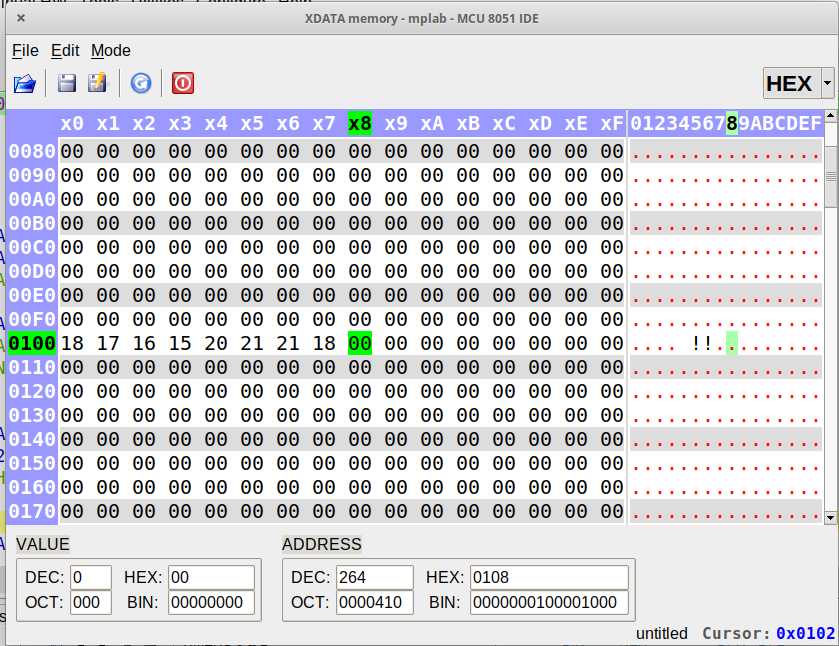
\includegraphics[width=\textwidth]{img/p29/ss1.png}
\end{center}
\begin{center}
	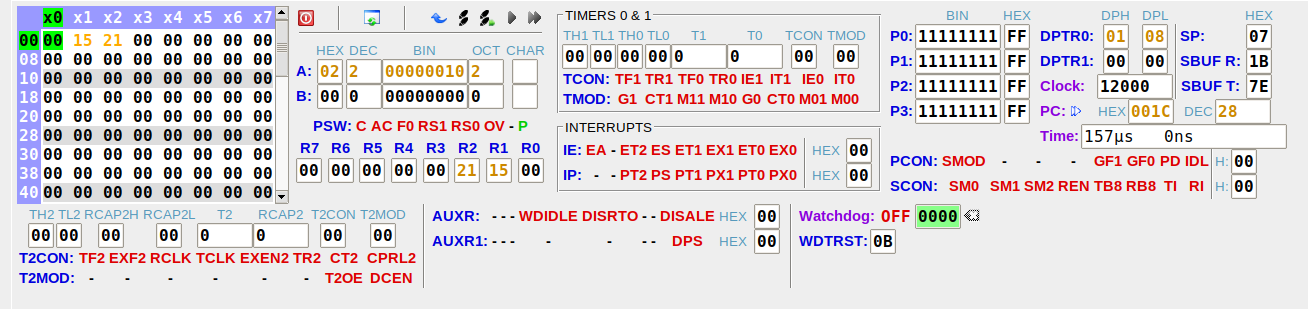
\includegraphics[width=\textwidth]{img/p29/ss2.png}
\end{center}


\subsection{Result}
Largest and smallest elements of an array was found on mcu8051ide